\chapter{Electrodynamics}
\label{p:em:ed12}



\section{Introduction}
In Grade 11 you learnt how a magnetic field is generated around a current carrying conductor. You also learnt how a current is generated in a conductor that moves in a magnetic field. This chapter describes how conductors moving in a magnetic field are applied in the real-world. 
\chapterstartvideo{VPpjl}
\section{Electrical machines - generators and motors}
%\begin{syllabus}
%\item Learners must be able to state that generators convert mechanical energy to electrical energy and motors convert electrical energy to mechanical energy
%\item Learners must be able to use Faraday's Law to explain why a current is induced in a coil that is rotated in a magnetic field.
%\item Learners must be able to use words and pictures to explain the basic principle of an AC generator (alternator) in which a coil is mechanically rotated in a magnetic field
%\item Learners must be able to use words and pictures to explain how a DC generator works and how it differs from an AC generator.
%\item Learners must be able to explain why a current-carrying coil placed in a magnetic field (but not parallel to the field) will turn by referring to the force exerted on moving charges by a magnetic field and the torque on the coil
%\item Learners must be able to use words and pictures to explain the basic principle of an electric motor.
%\item Learners must be able to give examples of the use of AC and DC generators.
%\item Learners must be able to give examples of the use of motors
%\end{syllabus}

We have seen that when a conductor is moved in a magnetic field or when a magnet is moved near a conductor, a current flows in the conductor. The amount of current depends on the speed at which the conductor experiences a changing magnetic field, the number of turns of the conductor and the position of the plane of the conductor with respect to the magnetic field. The effect of the orientation of the conductor with respect to the magnetic field is illustrated in Figure~\ref{fig:conductor}. 

\begin{figure}[htbp]
\begin{center}
\begin{pspicture}(0,0)(11,5)
%\psgrid[gridcolor=gray]
\def\magfieldF{\multirput(0,0)(0.25,0){9}{\psline{<-}(0,0)(0,2)}}
\def\magfieldT{\multirput(0,0)(0,0.25){9}{\multirput(0,0)(0.25,0){9}{\psdot[dotstyle=x](0,0)}}}
\def\frontview{\rput{0}{\psline[linewidth=0.1cm](1;180)(1;0)\psarc{->}{1}{0}{30}}}
\rput(0,3){\magfieldF\rput{0}(1,1){\frontview}}
\rput(0,0){\magfieldT\pscircle[linewidth=0.1cm](1,1){1}}

\rput(3,0)
{
\rput(0,3){\magfieldF\rput{45}(1,1){\frontview}}
\rput(0,0){\magfieldT\psellipse[linewidth=0.1cm](1,1)(0.5,1)}
}

\rput(6,0)
{
\rput(0,3){\magfieldF\rput{90}(1,1){\frontview}}
\rput(0,0){\magfieldT\rput(1,1){\psline[linewidth=0.1cm](1;270)(1;90)}}
}

\rput(9,0)
{
\rput(0,3){\magfieldF\rput{135}(1,1){\frontview}}
\rput(0,0){\magfieldT\psellipse[linewidth=0.1cm](1,1)(0.5,1)}
}

\uput[l](0,1){top view}
\uput[l](0,4){front view}
\rput(1,2.5){(a)}
\rput(4,2.5){(b)}
\rput(7,2.5){(c)}
\rput(10,2.5){(d)}
\end{pspicture}
\caption{Series of figures showing that the magnetic flux through a conductor is dependent on the angle that the plane of the conductor makes with the magnetic field. The greatest flux passes through the conductor when the plane of the conductor is perpendicular to the magnetic field  lines as in (a). The number of field lines passing through the conductor decreases, as the conductor rotates until it is parallel to the magnetic field (c).}
\label{fig:conductor}
\end{center}
\end{figure}

If the current flowing in the conductor were plotted as a function of the angle between the plane of the conductor and the magnetic field, then the current would vary as shown in Figure~\ref{fig:ac}. The current alternates about zero and is known as an \textit{alternating current} (abbreviated AC).


%%%% SARAH: Trying to remove the x axis numbers - they are irrelevant!
\begin{figure}[htbp]
\begin{center}
\begin{pspicture}(0,-2)(4.6,2)
%\psgrid[gridcolor=gray]
\psset{xunit=0.00556}
\psaxes[labels=none,ticks=none,dx=180,Dx=180]{<->}(0,0)(0,-1.5)(780,1.5)
\psplot{0}{720}{x sin}
\uput[r](780,0){time}
\uput[u](0,1.5){current (arbitrary units)}
\end{pspicture}
\caption{Variation of current as the angle of the plane of a conductor with the magnetic field changes.}
\label{fig:ac}
\end{center}
\end{figure}

Recall Faraday's Law which you learnt about in Grade 11:

\Definition{Faraday's Law}{The emf (electromotive force),
$\epsilon$, produced around a loop of conductor is proportional to
the rate of change of the magnetic flux, $\phi$, through the area,
$A$, of the loop. This can be stated mathematically as:
\begin{equation*}
\epsilon=-N\frac{\Delta \phi}{\Delta t}
\end {equation*}
 where $\phi=B\cdot A$ and $B$ is the strength of the magnetic field.}

Faraday's Law relates induced emf (electromotive force) to the rate of change of flux,
which is the product of the magnetic field and the cross-sectional
area the field lines pass through.
As the closed loop conductor changes orientation with respect to the magnetic field, the amount of magnetic flux through the area of the loop changes, and an emf is induced in the conducting loop. 


\subsection{Electrical generators}

\subsection*{AC generator}
The principle of rotating a conductor in a magnetic field is used in electrical generators. A generator converts mechanical energy (motion) into electrical energy.
 
\Definition{Generator}{A generator converts mechanical energy into electrical energy.}

The layout of a simple AC generator is shown in Figure~\ref{fig:ACgen}. The conductor in the shape of a coil is connected to a slip ring. The conductor is then manually rotated in the magnetic field generating an alternating emf. The slip rings are connected to the load via brushes.

\begin{figure}[htbp]
\begin{center}
%\begin{pspicture}(0,-2.2)(9,4)
%%\psgrid[gridcolor=gray]
%\psframe(0,2)(3,4)\uput[l](3,3){N}
%\psframe(6,2)(9,4)\uput[r](6,3){S}
%\psline[linearc=0.4cm](4.2,-1.4)(4.2,2)(3.4,2)(3.4,4)(5.6,4)(5.6,2)(4.8,2)(4.8,-0.4)
%\psframe*(4,-1)(5,-0.4)\psline(5,-0.4)(5,-1)\psline(5,-0.7)(6,-0.7)(6,0)(8,0)
%\psframe*(4,-2)(5,-1.4)\psline(5,-1.4)(5,-2)\psline(5,-1.7)(6,-1.7)(6,-2.2)(8,-2.2)
%\psframe[fillstyle=solid,fillcolor=lightgray](5,-1)(5.2,-0.4)\uput[u](5.2,-0.4){brush}
%\psframe[fillstyle=solid,fillcolor=lightgray](5,-2)(5.2,-1.4)\uput[d](5.2,-2){brush}
%\uput[l](4,-0.7){slip ring}
%\uput[l](4,-1.7){slip ring}
%\resistor[dipolestyle=zigzag](8,0)(8,-2.2){load}
%\rput(0,-1){\pscircle[linewidth=2pt](2,1){0.5}\uput[u](2,1.5){slip ring (front view)}}
%\end{pspicture}
\scalebox{1} % Change this value to rescale the drawing.
{
\begin{pspicture}(0,-3.041)(8.92,3.06)
\definecolor{color1802b}{rgb}{0.8,0.8,0.8}
\psframe[linewidth=0.042,dimen=outer](2.92,2.72)(0.04,0.86)
\psframe[linewidth=0.042,dimen=outer](8.8,2.7)(5.92,0.84)
\psbezier[linewidth=0.042](4.184828,-1.34)(4.0865517,0.88)(4.342069,0.8)(3.8310344,0.86)(3.32,0.92)(3.3396552,1.46)(3.3789656,2.14)(3.4182758,2.82)(4.08,2.68)(4.8727584,2.68)(5.6655173,2.68)(5.5,1.96)(5.5,1.48)(5.5,1.0)(5.4284515,1.0245473)(5.4,0.96)(5.371548,0.8954527)(5.0489655,0.86)(4.88,0.82)(4.7110343,0.78)(4.8334484,0.46)(4.7744827,-1.34)
\psframe[linewidth=0.042,dimen=outer,fillstyle=solid,fillcolor=black](5.06,-1.26)(3.78,-1.86)
\psframe[linewidth=0.042,dimen=outer,fillstyle=solid,fillcolor=color1802b](5.28,-1.18)(5.02,-1.92)
\psframe[linewidth=0.042,dimen=outer,fillstyle=solid,fillcolor=black](5.04,-2.36)(3.76,-2.96)
\psframe[linewidth=0.042,dimen=outer,fillstyle=solid,fillcolor=color1802b](5.26,-2.28)(5.0,-3.02)
\pscircle[linewidth=0.06,dimen=outer](1.41,-0.91){0.57}
\rput(2.5,1.765){N}
\rput(6.36,1.765){S}
\rput(5.34,-0.955){brush}
\rput(3.04,-1.595){slip ring}
\rput(3.06,-2.675){slip ring}
\rput(1.52,-0.135){slip ring (front view)}
\psline[linewidth=0.042cm,fillcolor=black](4.2,-1.82)(4.2,-2.4)
\psline[linewidth=0.042cm,fillcolor=black](5.26,-1.54)(6.04,-1.54)
\psline[linewidth=0.042cm,fillcolor=black](6.04,-1.54)(6.02,-0.84)
\psline[linewidth=0.042cm,fillcolor=black](6.02,-0.84)(7.84,-0.84)
\psline[linewidth=0.042cm,fillcolor=black](7.84,-0.84)(7.84,-1.5)
\psline[linewidth=0.042cm,fillcolor=black](7.84,-1.5)(8.08,-1.64)
\psline[linewidth=0.042cm,fillcolor=black](8.08,-1.64)(7.64,-1.8)
\psline[linewidth=0.042cm,fillcolor=black](7.64,-1.8)(8.08,-1.96)
\psline[linewidth=0.042cm,fillcolor=black](8.08,-1.96)(7.66,-2.16)
\psline[linewidth=0.042cm,fillcolor=black](7.66,-2.16)(8.08,-2.26)
\psline[linewidth=0.042cm,fillcolor=black](8.08,-2.26)(7.66,-2.46)
\psline[linewidth=0.042cm,fillcolor=black](7.66,-2.46)(7.86,-2.52)
\psline[linewidth=0.042cm,fillcolor=black](7.86,-2.52)(7.86,-3.02)
\psline[linewidth=0.042cm,fillcolor=black](7.86,-3.02)(5.96,-3.02)
\psline[linewidth=0.042cm,fillcolor=black](5.96,-3.02)(5.98,-2.64)
\psline[linewidth=0.042cm,fillcolor=black](5.98,-2.64)(5.26,-2.64)
\rput(8.57,-2.055){load}
\rput(5.11,0.545){coil}
\rput(1.47,2.905){magnet}
\rput(7.39,2.905){magnet}
\end{pspicture} 
}
\caption{Layout of an alternating current generator.}
\label{fig:ACgen}
\end{center}
\end{figure}

If a machine is constructed to rotate a magnetic field around a set of stationary wire coils with the turning of a shaft, AC voltage will be produced across the wire coils as that shaft is rotated, in accordance with Faraday's Law of electromagnetic induction. This is the basic operating principle of an AC generator.\\
 
In an AC generator the two ends of the coil are each attached to a slip ring that makes contact with brushes as the coil turns. The direction of the current changes with every half turn of the coil. As one side of the loop moves to the other pole of the magnetic field, the current in the loop changes direction. The two slip rings of the AC generator allow the coil to turn without breaking the connections to the load circuit. This type of current which changes direction is known as alternating current.\\  
 
\begin{IFact}{AC generators are also known as alternators. They are found in motor cars to charge the car battery.}
\end{IFact}

\subsection*{DC generator}
A simple DC generator is constructed the same way as an AC generator except that there is one slip ring which is split into two pieces, called a commutator, so the current in the external circuit does not change direction. The layout of a DC generator is shown in Figure~\ref{fig:DCgen}. The split-ring commutator accommodates for the change in direction of the current in the loop, thus creating direct current (DC) current going through the brushes and out to the circuit.

\begin{figure}[htbp]
\begin{center}
\begin{pspicture}(0,-2.2)(9,4)
%\psgrid[gridcolor=gray]
\psframe(0,2)(3,4)\uput[l](3,3){N}
\psframe(6,2)(9,4)\uput[r](6,3){S}
\psline[linearc=0.4cm](4.2,-0.4)(4.2,2)(3.4,2)(3.4,4)(5.6,4)(5.6,2)(4.8,2)(4.8,-0.4)
\psframe*(4,-1)(5,-0.4)\psline(5,-0.4)(5,-1)
\uput[d](4.4,-1){split ring}
\uput[ul](4,-0.4){brush}
\uput[ur](5,-0.4){brush}

\psframe[fillstyle=solid,fillcolor=lightgray](5,-1)(5.2,-0.4)\psline(5.2,-0.7)(6,-0.7)(6,0)(8,0)

\psframe[fillstyle=solid,fillcolor=lightgray](3.8,-1)(4,-0.4)\psline(3.8,-0.7)(3,-0.7)(3,-2.2)(8,-2.2)
\resistor[dipolestyle=zigzag](8,0)(8,-2.2){load}
\rput(0,-1){\psarc[linewidth=2pt](2,1){0.5}{0}{180}\psarc[linewidth=2pt](2,0.8){0.5}{180}{0}\uput[u](2,1.5){split ring commutator}}
\end{pspicture}
\caption{Layout of a direct current generator.}
\label{fig:DCgen}
\end{center}
\end{figure}

The shape of the emf from a DC generator is shown in Figure~\ref{fig:DCsignal}. The emf is not steady but is the absolute value of a sine/cosine wave.

%%% SARAH: Trying to remove x-axis numbering
\begin{figure}[htbp]
\begin{center}
\begin{pspicture}(0,-2)(4.6,2)
%\psgrid[gridcolor=gray]
\psset{xunit=0.00556}
\psaxes[labels=none,ticks=none,dx=180,Dx=180,label=0]{<->}(0,0)(0,-1.5)(780,1.5)
\def\sine{\psplot{0}{180}{x sin}}
\rput(0,0){\sine}
\rput(180,0){\sine}
\rput(360,0){\sine}
\rput(540,0){\sine}
\uput[r](780,0){$\theta$ or time}
\uput[u](0,1.5){current}
\end{pspicture}
\caption{Variation of emf in a DC generator.}
\label{fig:DCsignal}
\end{center}
\end{figure}

\subsection*{AC versus DC generators}

The problems involved with making and breaking electrical contact with a moving coil are sparking and heat, especially if the generator is turning at high speed. If the atmosphere surrounding the machine contains flammable or explosive vapours, the practical problems of spark-producing brush contacts are even greater.\\
 
If the magnetic field, rather than the coil/conductor is rotated, then brushes are not needed in an AC generator (alternator), so an alternator will not have the same problems as DC generators. 
The same benefits of AC over DC for generator design also apply to electric motors.
While DC motors need brushes to make electrical contact with moving coils of wire, AC motors do not. In fact, AC and DC motor designs are very similar to their generator counterparts. 
The AC motor is depends on the reversing magnetic field produced by alternating current through its stationary coils of wire to make the magnet rotate. The DC motor depends on the brush contacts making and breaking
connections to reverse current through the rotating coil every 1/2 rotation (180 degrees).


\subsection{Electric motors}
The basic principles of operation for a motor are the same as that of a generator, except that a motor converts electrical energy into mechanical energy (motion).

\Definition{Motor}{An electric motor converts electrical energy into mechanical energy.}

If one were to place a moving charged particle in a magnetic field, it would feel a force called the \textbf{Lorentz force}. 

\Definition{The Lorentz Force}{The Lorentz force is the force experienced by a moving charged particle in a magnetic field and can be described by:
\begin{equation*}
F = q \times v \times B
\end{equation*}
where \\
$F$ is the force (in newtons, N) \\
$q$ is the electric charge (in coulombs, C) \\
$v$ is the velocity of the charged particle (in $\rm{m.s^{-1}}$) and \\
$B$ is the magnetic field strength (in teslas, T). 
}

Current in a conductor consists of moving charges. Therefore, a current carrying coil in a magnetic field will also feel the Lorentz force. For a straight current carrying wire which is not moving:

\begin{equation*}
F = I \times L \times B
\end{equation*}
where \\
$F$ is the force (in newtons, N) \\
$I$ is the current in the wire (in amperes, A) \\
$L$ is the length of the wire which is in the magnetic field (in m) and \\
$B$ is the magnetic field strength (in teslas, T). \\

The direction of the Lorentz force is perpendicular to both the direction of the flow of current and the magnetic field and can be found using the \textbf{Right Hand Rule} as shown in the picture below. Use your \textit{right hand}; your thumb points in the direction of the current, your first finger in the direction of the magnetic field and your third finger will then point in the direction of the force.

\begin{center}
\scalebox{1}{% Change this value to rescale the drawing.
\begin{pspicture}(0,-2.8)(7.2617035,2.8)
\psline[linewidth=0.04cm](0.02,1.14)(1.42,1.14)
\psline[linewidth=0.04cm](1.42,1.14)(1.42,-0.84)
\psline[linewidth=0.04cm](1.42,-0.84)(0.0,-0.84)
\psline[linewidth=0.04cm](7.2182946,-0.8211864)(5.818297,-0.8187762)
\psline[linewidth=0.04cm](5.818297,-0.8187762)(5.8217053,1.1612209)
\psline[linewidth=0.04cm](5.8217053,1.1612209)(7.2417035,1.1587762)
\rput(1.14,0.125){S}
\rput(6.14,0.165){N}
\pscircle[linewidth=0.04,dimen=outer](4.07,0.13){0.21}
\pscircle[linewidth=0.04,dimen=outer](4.21,0.05){0.01}
\rput(4.08,0.105){+}
\psline[linewidth=0.054cm,arrowsize=0.05291667cm 2.0,arrowlength=1.4,arrowinset=0.4]{->}(3.96,-0.02)(2.26,-2.24)
\psline[linewidth=0.054cm,arrowsize=0.05291667cm 2.0,arrowlength=1.4,arrowinset=0.4]{->}(3.9,0.18)(1.5,0.18)
\psline[linewidth=0.054cm,arrowsize=0.05291667cm 2.0,arrowlength=1.4,arrowinset=0.4]{->}(4.06,0.32)(4.06,2.7)
\rput(0.63,1.345){magnet}
\rput(6.53,1.365){magnet}
\rput(5.65,2.625){\small Direction of current }
\rput(4.98,2.305){\small in the wire}
\rput(4.89,1.94){\footnotesize [THUMB]}
\rput(3.41,-2.58){\footnotesize [2nd FINGER]}
\rput(4.63,-2.195){\small Direction of the Lorentz force}
\rput(2.65,0.765){\small Direction of the }
\rput(2.58,0.445){\small magnetic field}
\rput(2.43,-0.18){\footnotesize [1st FINGER]}
\end{pspicture} 
}
\end{center}

Both motors and generators can be explained in terms of a coil that rotates in a magnetic field. In a generator the coil is attached to an external circuit that is turned, resulting in a changing flux that induces an emf. In a motor, a current-carrying coil in a magnetic field experiences a force on both sides of the coil, creating a twisting force (called a \textit{torque}, pronounce like 'talk') which makes it turn.\\

Any coil carrying current can feel a force in a magnetic field. The force is the Lorentz force on the moving charges in the conductor. The force on opposite sides of the coil will be in opposite directions because the charges are moving in opposite directions. This means the coil will rotate, see the picture below:

\begin{center}
\scalebox{1} % Change this value to rescale the drawing.
{
\begin{pspicture}(0,-2.32)(7.96,2.32)
\definecolor{color0}{rgb}{0.6,0.6,0.6}
\psline[linewidth=0.04cm,linecolor=color0,arrowsize=0.05291667cm 4.0,arrowlength=1.4,arrowinset=0.4]{->}(0.9,1.94)(0.9,-1.74)
\psline[linewidth=0.04cm,linecolor=color0,arrowsize=0.05291667cm 4.0,arrowlength=1.4,arrowinset=0.4]{->}(1.5,1.94)(1.5,-1.74)
\psline[linewidth=0.04cm,linecolor=color0,arrowsize=0.05291667cm 4.0,arrowlength=1.4,arrowinset=0.4]{->}(2.12,1.92)(2.12,-1.76)
\psline[linewidth=0.04cm,linecolor=color0,arrowsize=0.05291667cm 4.0,arrowlength=1.4,arrowinset=0.4]{->}(2.72,1.94)(2.72,-1.74)
\psline[linewidth=0.04cm,linecolor=color0,arrowsize=0.05291667cm 4.0,arrowlength=1.4,arrowinset=0.4]{->}(3.32,1.92)(3.32,-1.76)
\psline[linewidth=0.04cm,linecolor=color0,arrowsize=0.05291667cm 4.0,arrowlength=1.4,arrowinset=0.4]{->}(3.92,1.92)(3.92,-1.76)
\psline[linewidth=0.04cm,linecolor=color0,arrowsize=0.05291667cm 4.0,arrowlength=1.4,arrowinset=0.4]{->}(4.5,1.92)(4.5,-1.76)
\psline[linewidth=0.04cm,linecolor=color0,arrowsize=0.05291667cm 4.0,arrowlength=1.4,arrowinset=0.4]{->}(5.12,1.94)(5.12,-1.74)
\psline[linewidth=0.04cm,linecolor=color0,arrowsize=0.05291667cm 4.0,arrowlength=1.4,arrowinset=0.4]{->}(5.72,1.94)(5.72,-1.74)
\psline[linewidth=0.04cm,linecolor=color0,arrowsize=0.05291667cm 4.0,arrowlength=1.4,arrowinset=0.4]{->}(6.32,1.94)(6.32,-1.74)
\psline[linewidth=0.04](0.34,0.22)(1.88,0.22)(2.26,1.16)(6.16,1.16)(5.64,-1.1)(1.42,-1.08)(1.76,0.0)(0.24,0.0)
\psellipse[linewidth=0.04,linecolor=color0,dimen=outer](6.99,0.16)(0.39,1.0)
\psbezier[linewidth=0.04,arrowsize=0.05291667cm 4.0,arrowlength=1.4,arrowinset=0.4]{->}(7.34,0.04)(7.36,0.06)(7.3,-0.86)(7.0142856,-0.82)(6.7285714,-0.78)(6.614286,-0.33518797)(6.6714287,0.46)(6.7285714,1.255188)(7.16,1.32)(7.36,0.54)
\psline[linewidth=0.04cm,arrowsize=0.05291667cm 3.0,arrowlength=1.4,arrowinset=0.4]{->}(3.46,1.16)(4.66,1.16)
\psline[linewidth=0.04cm,arrowsize=0.05291667cm 3.0,arrowlength=1.4,arrowinset=0.4]{->}(4.7,-1.1)(3.5,-1.1)
\psframe[linewidth=0.02,linecolor=color0,dimen=outer](2.96,0.38)(2.74,0.14)
\psline[linewidth=0.12cm,arrowsize=0.05291667cm 2.0,arrowlength=1.4,arrowinset=0.4]{->}(4.02,1.14)(4.76,1.62)
\psline[linewidth=0.12cm,arrowsize=0.05291667cm 2.0,arrowlength=1.4,arrowinset=0.4]{->}(3.32,-1.08)(2.68,-1.62)
\psline[linewidth=0.12cm,arrowsize=0.05291667cm 2.0,arrowlength=1.4,arrowinset=0.4]{->}(2.1,0.66)(1.56,0.66)
\psline[linewidth=0.12cm,arrowsize=0.05291667cm 2.0,arrowlength=1.4,arrowinset=0.4]{->}(1.6,-0.62)(1.06,-0.62)
\psline[linewidth=0.12cm,arrowsize=0.05291667cm 2.0,arrowlength=1.4,arrowinset=0.4]{->}(6.02,0.66)(6.56,0.66)
\psline[linewidth=0.12cm,arrowsize=0.05291667cm 2.0,arrowlength=1.4,arrowinset=0.4]{->}(5.7,-0.64)(6.24,-0.64)
\rput(5.12,2.125){resultant force is \textit{into} the page}
\rput(2.95,-2.095){resultant force is \textit{out of} the page}
\psline[linewidth=0.02cm](0.04,0.14)(7.72,0.14)
\end{pspicture} 
}

\end{center}

 
Instead of rotating the loops through a magnetic field to create electricity, a current is sent through the wires, creating electromagnets. The outer magnets will then repel the electromagnets and rotate the shaft as an electric motor. If the current is AC, the two slip rings are required to create an AC motor. An AC motor is shown in Figure~\ref{fig:ACmotor} 

\begin{figure}[H]
\begin{center}
%\begin{pspicture}(0,-2.2)(9,4)
%%\psgrid[gridcolor=gray]
%\psframe(0,2)(3,4)\uput[l](3,3){N}
%\psframe(6,2)(9,4)\uput[r](6,3){S}
%\psline[linearc=0.4cm](4.2,-1.4)(4.2,2)(3.4,2)(3.4,4)(5.6,4)(5.6,2)(4.8,2)(4.8,-0.4)
%\psframe*(4,-1)(5,-0.4)\psline(5,-0.4)(5,-1)\psline(5,-0.7)(6,-0.7)(6,0)(8,0)
%\psframe*(4,-2)(5,-1.4)\psline(5,-1.4)(5,-2)\psline(5,-1.7)(6,-1.7)(6,-2.2)(8,-2.2)
%\psframe[fillstyle=solid,fillcolor=lightgray](5,-1)(5.2,-0.4)\uput[u](5.2,-0.4){brush}
%\psframe[fillstyle=solid,fillcolor=lightgray](5,-2)(5.2,-1.4)\uput[d](5.2,-2){brush}
%\uput[l](4,-0.7){slip ring}
%\uput[l](4,-1.7){slip ring}
%\battery(8,0)(8,-2.2){}
%\rput(0,-1){\pscircle[linewidth=2pt](2,1){0.5}\uput[u](2,1.5){slip ring (front view)}}
%\end{pspicture}
\scalebox{1} % Change this value to rescale the drawing.
{
\begin{pspicture}(0,-3.041)(8.8,3.06)
\definecolor{color1802b}{rgb}{0.8,0.8,0.8}
\psframe[linewidth=0.042,dimen=outer](2.92,2.72)(0.04,0.86)
\psframe[linewidth=0.042,dimen=outer](8.8,2.7)(5.92,0.84)
\psbezier[linewidth=0.042](4.184828,-1.34)(4.0865517,0.88)(4.342069,0.8)(3.8310344,0.86)(3.32,0.92)(3.3396552,1.46)(3.3789656,2.14)(3.4182758,2.82)(4.08,2.68)(4.8727584,2.68)(5.6655173,2.68)(5.5,1.96)(5.5,1.48)(5.5,1.0)(5.4284515,1.0245473)(5.4,0.96)(5.371548,0.8954527)(5.0489655,0.86)(4.88,0.82)(4.7110343,0.78)(4.8334484,0.46)(4.7744827,-1.34)
\psframe[linewidth=0.042,dimen=outer,fillstyle=solid,fillcolor=black](5.06,-1.26)(3.78,-1.86)
\psframe[linewidth=0.042,dimen=outer,fillstyle=solid,fillcolor=color1802b](5.28,-1.18)(5.02,-1.92)
\psframe[linewidth=0.042,dimen=outer,fillstyle=solid,fillcolor=black](5.04,-2.36)(3.76,-2.96)
\psframe[linewidth=0.042,dimen=outer,fillstyle=solid,fillcolor=color1802b](5.26,-2.28)(5.0,-3.02)
\pscircle[linewidth=0.06,dimen=outer](1.41,-0.91){0.57}
\rput(2.5,1.765){N}
\rput(6.36,1.765){S}
\rput(5.34,-0.955){brush}
\rput(3.04,-1.595){slip ring}
\rput(3.06,-2.675){slip ring}
\rput(1.52,-0.135){slip ring (front view)}
\psline[linewidth=0.042cm,fillcolor=black](4.2,-1.82)(4.2,-2.4)
\psline[linewidth=0.042cm,fillcolor=black](5.26,-1.54)(6.04,-1.54)
\psline[linewidth=0.042cm,fillcolor=black](6.04,-1.54)(6.02,-0.84)
\psline[linewidth=0.042cm,fillcolor=black](6.02,-0.84)(7.84,-0.84)
\psline[linewidth=0.042cm,fillcolor=black](7.84,-0.84)(7.84,-1.5)
\psline[linewidth=0.042cm,fillcolor=black](7.86,-2.52)(7.86,-3.02)
\psline[linewidth=0.042cm,fillcolor=black](7.86,-3.02)(5.96,-3.02)
\psline[linewidth=0.042cm,fillcolor=black](5.96,-3.02)(5.98,-2.64)
\psline[linewidth=0.042cm,fillcolor=black](5.98,-2.64)(5.26,-2.64)
\rput(5.11,0.545){coil}
\rput(1.47,2.905){magnet}
\rput(7.39,2.905){magnet}
\psframe[linewidth=0.042,dimen=outer](8.68,-1.52)(7.62,-2.54)
\rput(8.11,-1.855){\scriptsize AC}
\rput(8.16,-2.095){\scriptsize source}
\end{pspicture} 
}
\caption{Layout of an alternating current motor.}
\label{fig:ACmotor}
\end{center}
\end{figure}

If the current is DC, split-ring commutators are required to create a DC motor. This is shown in Figure~\ref{fig:DCmotor}.

\begin{figure}[H]
\begin{center}
\begin{pspicture}(0,-2.2)(9,4)
%\psgrid[gridcolor=gray]
\psframe(0,2)(3,4)\uput[l](3,3){N}
\psframe(6,2)(9,4)\uput[r](6,3){S}
\psline[linearc=0.4cm](4.2,-0.4)(4.2,2)(3.4,2)(3.4,4)(5.6,4)(5.6,2)(4.8,2)(4.8,-0.4)
\psframe*(4,-1)(5,-0.4)\psline(5,-0.4)(5,-1)
\uput[d](4.4,-1){split ring}
\uput[ul](4,-0.4){brush}
\uput[ur](5,-0.4){brush}

\psframe[fillstyle=solid,fillcolor=lightgray](5,-1)(5.2,-0.4)\psline(5.2,-0.7)(6,-0.7)(6,0)(8,0)

\psframe[fillstyle=solid,fillcolor=lightgray](3.8,-1)(4,-0.4)\psline(3.8,-0.7)(3,-0.7)(3,-2.2)(8,-2.2)
\battery(8,0)(8,-2.2){}
\rput(0,-1){\psarc[linewidth=2pt](2,1){0.5}{0}{180}\psarc[linewidth=2pt](2,0.8){0.5}{180}{0}\uput[u](2,1.5){split ring commutator}}
\end{pspicture}
\caption{Layout of a direct current motor.}
\label{fig:DCmotor}
\end{center}
\end{figure}


\subsection{Real-life applications}

\subsubsection{Cars}
A car contains an alternator that charges its battery and powers the car's electric system when its engine is running. Alternators have the great advantage over direct-current generators of not using a commutator, which makes them simpler, lighter, less costly, and more rugged than a DC generator.

\Activity{Research Topic}{Alternators}
{Try to find out the different ampere values produced by alternators for different types of machines. Compare these to understand what numbers make sense in the real world. You will find different numbers for cars, trucks, buses, boats etc. Try to find out what other machines might have alternators.
}

A car also contains a DC electric motor, the starter motor, to turn over the engine to start it.
A starter motor consists of the very powerful DC electric motor and starter solenoid that is attached to the motor.
A starter motor requires a very high current to crank the engine, that's why it's connected to the battery with large cables. 

\subsubsection{Electricity Generation}

AC generators are mainly used in the real-world to generate electricity.\\
 
\begin{figure}[htbp]
\begin{center}
\begin{pspicture}(-5,-3)(5,3)
%\psgrid
\rput(0,0){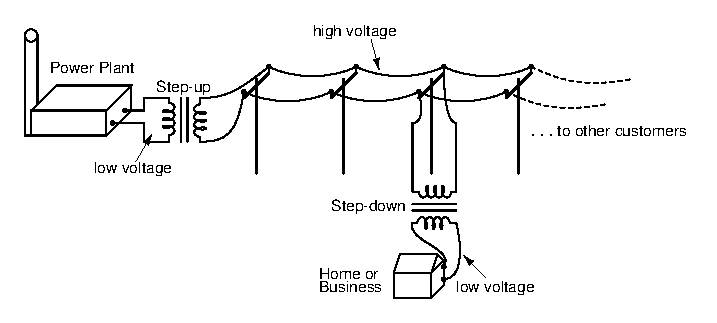
\includegraphics{../../epsimages/02007.eps}}
\end{pspicture}
\caption{AC generators are used at the power plant to generate electricity.}
\end{center}
\end{figure}

\Exercise{generators and motors}{
\begin{enumerate}
\item State the difference between a generator and a motor.
\item Use Faraday's Law to explain why a current is induced in a coil that is rotated in a magnetic field.
\item Explain the basic principle of an AC generator in which a coil is mechanically rotated in a magnetic field. Draw a diagram to support your answer.
\item  Explain how a DC generator works. Draw a diagram to support your answer. Also, describe how a DC generator differs from an AC generator.
\item  Explain why a current-carrying coil placed in a magnetic field (but not parallel to the field) will turn. Refer to the force exerted on moving charges by a magnetic field and the torque on the coil.
\item  Explain the basic principle of an electric motor. Draw a diagram to support your answer.
\item  Give examples of the use of AC and DC generators.
\item  Give examples of the uses of motors.
\end{enumerate}
% Automatically inserted shortcodes - number to insert 8
\par \practiceinfo
\par \begin{tabular}[h]{cccccc}
% Question 1
(1.)	01yd	&
% Question 2
(2.)	01ye	&
% Question 3
(3.)	01yf	&
% Question 4
(4.)	01yg	&
% Question 5
(5.)	01yh	&
% Question 6
(6.)	01yi	\\ % End row of shortcodes
% Question 7
(7.)	01yj	&
% Question 8
(8.)	01yk	&
\end{tabular}
% Automatically inserted shortcodes - number inserted 8
}

\section{Alternating Current}
%\begin{syllabus}
%\item Learners must be able to Explain the advantages of alternating current
%\item Learners must be able to Write expressions for the current and voltage in an AC circuit
%\item Learners must be able to Define the rms (root mean square) values for current and voltage as Irms.  =   and Vrms.  =  respectively, and explain why these values are useful.
%\item Learners must be able to Draw a graph of voltage vs time and current vs time for an AC circuit.
%\item Note: The main advantage to AC is that the voltage can be changed using transformers.  That means that the voltage can be stepped up at power stations to a very high voltage so that electrical energy can be transmitted along power lines at low current and therefore experience low energy loss due to heating.  The voltage can then be stepped down for use in buildings, street lights, and so forth.
%\end{syllabus}

Most students learning about electricity begin with what is known as \textit{direct current} (DC), which is electricity flowing in a constant direction. DC is the kind of electricity made by a battery, with definite positive and negative terminals.\\ 
 
However, we have seen that the electricity produced by some generators alternates and is therefore known as \textit{alternating current} (AC). The main advantage to AC is that the voltage can be changed using transformers.  That means that the voltage can be stepped up at power stations to a very high voltage so that electrical energy can be transmitted along power lines at low current and therefore experience low energy loss due to heating.  The voltage can then be stepped down for use in buildings and street lights.

\begin{IFact}{In South Africa alternating current is generated at a frequency of 50~Hz.}\end{IFact}

The circuit symbol for alternating current is:
\begin{center}
\begin{pspicture}(0,0)(2,2)
\Ucc[labeloffset=0](0,1)(2,1){\Huge $\sim$}
\end{pspicture}
\end{center}

Graphs of voltage against time and current against time for an AC circuit are shown in Figure~\ref{fig:ACgraphs}

%%% SARAH: Get rid of the numbering on the x axis!!!
\begin{figure}[htbp]
\begin{center}
\begin{pspicture}(0,-2)(4.6,2)
%\psgrid[gridcolor=gray]
\psset{xunit=0.00556}
\psaxes[labels=none,ticks=none,dx=180,Dx=180]{<->}(0,0)(0,-1.5)(780,1.5)
\psplot{0}{720}{x sin}
\uput[r](780,0){time}
\uput[u](0,1.5){current OR voltage}
\end{pspicture}
\caption{Graph of current or voltage in an AC circuit.}
\label{fig:ACgraphs}
\end{center}
\end{figure}

In an ideal DC circuit the current and voltage are constant. In an AC circuit the current and voltage vary with time. The value of the current or voltage at any specific time is called the \textit{instantaneous current or voltage} and is calculated as follows:
\begin{eqnarray*}
i&=&I_{max}\sin(2\pi f t + \phi)\\
v&=&V_{max}\sin(2\pi f t)
\end{eqnarray*}
 $i$ is the instantaneous current. $I_{max}$ is the maximum current. $v$ is the instantaneous voltage. $V_{max}$ is the maximum voltage. $f$ is the frequency of the AC and $t$ is the time at which the instantaneous current or voltage is being calculated.\\
The average value we use for AC is known as the root mean square (rms) average. This is defined as:
\begin{eqnarray*}
I_{rms}&=&\frac{I_{max}}{\sqrt{2}}\\
V_{rms}&=&\frac{V_{max}}{\sqrt{2}}
\end{eqnarray*}
Since AC varies sinusoidally, with as much positive as negative, doing a straight average would get you zero for the average voltage. The rms value by-passes this problem.

\Exercise{alternating  current}{
\begin{enumerate}
\item Explain the advantages of alternating current.
\item Write expressions for the current and voltage in an AC circuit.
\item Define the rms (root mean square) values for current and voltage for AC.
\item What is the period of the AC generated in South Africa?
\item If $V_{max}$ at a power station generator is 340~V AC, what is the mains supply (rms voltage) in our household?
\item Draw a graph of voltage vs time and current vs time for an AC circuit.
\end{enumerate}

% Automatically inserted shortcodes - number to insert 6
\par \practiceinfo
\par \begin{tabular}[h]{cccccc}
% Question 1
(1.)	01ym	&
% Question 2
(2.)	01yn	&
% Question 3
(3.)	01yp	&
% Question 4
(4.)	01yq	&
% Question 5
(5.)	01yr	&
% Question 6
(6.)	01ys	\\ % End row of shortcodes
\end{tabular}
% Automatically inserted shortcodes - number inserted 6

}

\section{Capacitance and inductance}
%\begin{syllabus}
%\item The learner must be able to Revise capacitance from Grade 11
%\item The learner must be able to Define the reactance of a capacitor as $X_C=\frac{1}{2\pi fC}$  where reactance in an AC circuit plays a similar role to resistance in a DC circuit
%\item The learner must be able to Explain that a capacitor blocks the flow of DC and low frequency AC but allows the flow of high frequency AC because its reactance decreases with increasing frequency.
%\item The learner must be able to Describe an inductor as a solenoid, and inductance, L, as the ability of the solenoid to create an induced voltage when a changing current passes through it
%\item The learner must be able to Define the reactance of an inductor as $X_L = 2\pi fL$
%\item The learner must be able to Calculate the inductance of a solenoid using the expression $L=\frac{\mu_0 A N^2}{l}$, where inductance is measured in henry (H).
%\item The learner must be able to Explain that an inductor blocks high frequency AC because its reactance increases with frequency, but allows low frequency AC and DC to pass.
%\end{syllabus}

Capacitors and inductors are found in many circuits. Capacitors store an electric field, and are used as temporary power sources as well as to minimise power fluctuations in major circuits. Inductors work in conjunction with capacitors for electrical signal processing. Here we explain the physics and applications of both.

\subsection{Capacitance}
You have learnt about capacitance and capacitors in Grade 11. %Please read through Chapter~\ref{p:em:es11:c} to recap what you learnt about capacitance in a DC circuit.\\ 
 
In this section you will learn about capacitance in an AC circuit. A capacitor in an AC circuit has \textit{reactance}. Reactance in an AC circuit plays a similar role to resistance in a DC circuit. The reactance of a capacitor $X_C$ is defined as:\\
\begin{equation*}
X_C=\frac{1}{2\pi fC}
\end{equation*}
where $C$ is the capacitance and $f$ is the AC frequency.\\
 
If we examine the equation for the reactance of a capacitor, we see that the frequency is in the denominator. Therefore, when the frequency is low, the capacitive reactance is very high. This is why a capacitor blocks the flow of DC and low frequency AC because its reactance increases with decreasing frequency.\\ 
 
When the frequency is high, the capacitive reactance is low. This is why a capacitor allows the flow of high frequency AC because its reactance decreases with increasing frequency.



\subsection{Inductance}

Inductance (measured in henries, symbol H) is a measure of the generated emf for a unit change in current. For example, an inductor with an inductance of 1~H produces an emf of 1~V when the current through the inductor changes at the rate of 1~A$\cdot$s$^{-1}$.\\ 

An inductor is a passive electrical device used in electrical circuits for its property of inductance. An inductor is usually made as a coil (or solenoid) of conducting material, typically copper wire, wrapped around a core either of air or of ferromagnetic material.\\ 
 
Electrical current through the conductor creates a magnetic flux proportional to the current. A change in this current creates a change in magnetic flux that, in turn, generates an emf that acts to oppose this change in current.\\ 

 
The inductance of an inductor is determined by several factors:
\begin{itemize}
\item the shape of the coil; a short, fat coil has a higher inductance than one that is thin and tall.
\item the material that the conductor is wrapped around. 
\item how the conductor is wound; winding in opposite directions will cancel out the inductance effect, and you will have only a resistor.
\end{itemize}

The inductance of a solenoid is defined by:\\
 \begin{equation*}
L=\frac{\mu_0 A N^2}{l}
 \end{equation*}
where $\mu_0$ is the permeability of the core material (in this case air), $A$ is the cross-sectional area of the solenoid, $N$ is the number of turns and $l$ is the length of the solenoid. 

\Definition{Permeability}{Permeability is the property of a material which describes the magnetisation developed in that material when excited by a source.}

\begin{IFact}{The permeability of free space is $4 \pi \times 10^{-7}$ henry per metre.}
\end{IFact}

\begin{wex}{Inductance I}{Determine the inductance of a coil with a core material of air. A cross-sectional area of $0,3\rm{m^2}$, with 1000 turns and a length of 0,1~m}
{
\westep{Determine how to approach the problem}
We are calculating inductance, so we use the equation:
\begin{eqnarray*}
L=\frac{\mu_0 A N^2}{l}\\
\end{eqnarray*}\\
The permeability is that for free space:$4 \pi \textrm{x} 10^{-7}$ henry per metre.

\westep{Solve the problem}
\begin{eqnarray*}
L&=&\frac{\mu_0 A N^2}{l}\\
&=&\frac{(4 \pi \times 10^{-7})(0,3)(1000)}{0,1}\\ 
&=&3,8 \times 10^{-3} \textrm H/m\\
\end{eqnarray*}

\westep{Write the final answer}
The inductance of the coil is $3,8\times 10^{-3}$~H/m.}
\end{wex}


\begin{wex}{Inductance II}{Calculate the inductance of a 5~cm long solenoid with a diameter of 4~mm and 2000 turns.}
{Again this is an inductance problem, so we use the same formula as the worked example above.\\
 
$$\textrm{r} = \frac{4 \textrm{ mm}}{2} = 2 \textrm{ mm} = 0,002 \textrm{ m}$$
$$\textrm{A} = \pi \textrm{r}^2 = \pi \times 0,002^2$$

\begin{eqnarray*}
\textrm{L} & = & \frac{\mu_0 \textrm{A} \textrm{N}^2}{l}\\
& = & \frac{4 \pi \times 10^{-7} \times 0,002^2 \times \pi \times 2000^2}{0,05}\\
& = & 0,00126 \textrm{ H}\\
& = & 1,26\textrm{ mH}\\
\end{eqnarray*}
}

\end{wex}

An inductor in an AC circuit also has a reactance, $X_L$. Reactance is the property of an inductor that opposes the flow of AC current. Reactance is defined by:
\begin{equation*}
X_L = 2\pi fL
\end{equation*}
where $L$ is the inductance and $f$ is the frequency of the AC.
 
If we examine the equation for the reactance of an inductor, we see that inductive reactance increases with increasing frequency. Therefore, when the frequency is low, the inductive reactance is very low. This is why an inductor allows the flow of DC and low frequency AC: its reactance decreases with decreasing frequency.
 
When the frequency is high, the inductive reactance is high. This is why an inductor blocks the flow of high frequency AC because its reactance increases with increasing frequency.

\Exercise{capacitance and inductance}{
\begin{enumerate}
\item Describe what is meant by reactance.
\item Define the reactance of a capacitor.
\item Explain how a capacitor blocks the flow of DC and low frequency AC but allows the flow of high frequency AC.
\item Describe what is an inductor.
\item Describe what is inductance.
\item What is the unit of inductance?
\item Define the reactance of an inductor.
\item Write the equation describing the inductance of a solenoid.
\item Explain how an inductor blocks high frequency AC, but allows low frequency AC and DC to pass.
\end{enumerate}
% Automatically inserted shortcodes - number to insert 9
\par \practiceinfo
\par \begin{tabular}[h]{cccccc}
% Question 1
(1.)	01yt	&
% Question 2
(2.)	01yu	&
% Question 3
(3.)	01yv	&
% Question 4
(4.)	01yw	&
% Question 5
(5.)	01yx	&
% Question 6
(6.)	01yy	\\ % End row of shortcodes
% Question 7
(7.)	01yz	&
% Question 8
(8.)	01z0	&
% Question 9
(9.)	01z1	&
\end{tabular}
% Automatically inserted shortcodes - number inserted 9
}

\summary{VPpkc}
\begin{itemize}
\item Electrical generators convert mechanical energy into electrical energy.
\item Electric motors convert electrical energy into mechanical energy.
\item There are two types of generators - AC and DC. An AC generator is also called an alternator.
\item There are two types of motors - AC and DC.
\item Alternating current (AC) has many advantages over direct current (DC).
\item Capacitors and inductors are important components in an AC circuit.
\item The reactance of a capacitor or inductor is affected by the frequency of the AC.
\end{itemize}

\begin{eocexercises}{}
\begin{enumerate}
\item{[SC 2003/11] Explain the difference between alternating current (AC) and direct current (DC).}

\item Explain how an AC generator works. You may use sketches to support your answer.

\item What are the advantages of using an AC motor rather than a DC motor.

\item Explain how a DC motor works.
 
\item At what frequency is AC generated by Eskom in South Africa?

\item (IEB 2001/11 HG1) - \textbf{Work, Energy and Power in Electric Circuits}\\
Mr. Smith read through the agreement with Eskom (the electricity provider). He found out that alternating current is supplied to his house at a frequency of 50 Hz. He then consulted a book on electric current, and discovered that alternating current moves to and fro in the conductor. So he refused to pay his Eskom bill on the grounds that every electron that entered his house would leave his house again, so therefore Eskom had supplied him with nothing!\\
 
Was Mr. Smith correct? Or has he misunderstood something about what he is paying for? Explain your answer briefly.
 

\item What do we mean by the following terms in electrodynamics?
\begin{enumerate}
\item inductance
\item reactance
\item solenoid
\item permeability

\end{enumerate}

\end{enumerate}


% Automatically inserted shortcodes - number to insert 7
\par \practiceinfo
\par \begin{tabular}[h]{cccccc}
% Question 1
(1.)	01iy	&
% Question 2
(2.)	01iz	&
% Question 3
(3.)	01j0	&
% Question 4
(4.)	01j1	&
% Question 5
(5.)	01j2	&
% Question 6
(6.)	01j3	\\ % End row of shortcodes
% Question 7
(7.)	01j4	&
\end{tabular}
% Automatically inserted shortcodes - number inserted 7
\end{eocexercises}

% CHILD SECTION END 



% CHILD SECTION START 

\setlength{\parskip}{2ex}

